\documentclass[a4paper, 12pt]{article}
\usepackage[english]{babel}
\usepackage[utf8]{inputenc}
\usepackage[T1]{fontenc}
\usepackage{lmodern}
\usepackage{hyperref}
\usepackage[numbers, sort&compress]{natbib}
\usepackage{calc}
\usepackage{fancyhdr}
\usepackage{graphics}
\usepackage{nowidow}
\usepackage{color}
\usepackage{subcaption}
\usepackage{enumitem}
\usepackage{epsfig}
\usepackage{epstopdf}


\newlength{\oneLine}
\newlength{\halfLine}
\setlength{\oneLine}{12pt}
\setlength{\halfLine}{6pt}

\newlength{\eqMargin}
\newlength{\eqHorizMargin}
\newlength{\eqVertMargin}

\setlength{\eqMargin}{20mm}
\setlength{\eqHorizMargin}{\eqMargin}
\setlength{\eqVertMargin}{\eqMargin}

% Paper
\setlength{\paperwidth}{210mm}
\setlength{\paperheight}{297mm}

% Rid the extra space
\setlength{\hoffset}{-1in}
\setlength{\voffset}{-1in}
\addtolength{\hoffset}{\eqHorizMargin}
\addtolength{\voffset}{\eqVertMargin}

% Set margin from the page border (horizontal)
\setlength{\oddsidemargin}{0pt}
\setlength{\evensidemargin}{0pt}

% Header
\setlength{\topmargin}{0pt}
\setlength{\headheight}{42pt}
\setlength{\headsep}{18pt}
\renewcommand{\headrulewidth}{0pt}

% Footer
\addtolength{\footskip}{18pt}
\renewcommand{\footrulewidth}{0pt}

% Margin notes
\setlength{\marginparsep}{0pt}
\setlength{\marginparwidth}{0pt}

% Text
\setlength{\textwidth}{\paperwidth - \hoffset - \hoffset - 25.4mm - 25.4mm}
\setlength{\textheight}{\paperheight - \voffset - \topmargin - \headheight - \headsep - \footskip - \voffset - 25.4mm - 25.4mm}

%\setlength{\labelwidth}{20mm}

% Hyperref settings
\hypersetup{
    unicode=true,					% non-Latin characters in Acrobat's bookmarks
    pdftoolbar=true,				% show Acrobat's toolbar?
    pdfmenubar=true,				% show Acrobat's menu?
    pdffitwindow=false,				% window fit to page when opened
    pdfstartview={FitH},			% fits the width of the page to the window
    pdftitle={S-26.3120 Radio Engineering, laboratory course},	% title
    pdfauthor={Tuomas Leinonen} {Sampo Salo} {Huy Nguyen},	% author
    pdfsubject={Radio Engineering},	% subject of the document
    pdfcreator={LaTeX},				% creator of the document
    pdfproducer={Aalto},			% producer of the document
    pdfkeywords={radio} {gsm} {bs} {tx},	% list of keywords
    pdfnewwindow=true,				% links in new window
    colorlinks=true,				% false: boxed links; true: colored links
    linkcolor=black,				% color of internal links
    citecolor=black,				% color of links to bibliography
    filecolor=black,				% color of file links
    urlcolor=black					% color of external links
}

% Bad hyphenation
%\hyphenation{}

\definecolor{dkred}{rgb}{0.6, 0, 0}
\definecolor{dkgrn}{rgb}{0, 0.6, 0}
\definecolor{dkblue}{rgb}{0, 0, 0.6}

\pagestyle{fancy}
\lhead{S-26.3120 Radio Engineering, laboratory course\\Lab 2: GSM Base Station Receiver -- Pre-study report\\}
\rhead{Sampo Salo, 79543L\\Tuomas Leinonen, 84695P\\Huy Nguyen, 12345A}
\cfoot{\thepage}


\begin{document}

\begin{titlepage}
\pagestyle{empty}
\begin{center}

\vspace*{30mm}
\noindent\LARGE{\textbf{S-26.3120 Radio Engineering, laboratory course}}

\vspace*{20mm}

\Large{\textbf{Lab 2: GSM Base Station Receiver}}\\

\vspace*{15mm}

\large{\textbf{Pre-study report}}\\
\vspace{15mm}
\large{\today}
	
\vspace*{30mm}
\large{
	\begin{tabular}{l l}
		\textbf{Group 3:} 	& \\
		Sampo Salo			& 79543L	\\
		Tuomas Leinonen 	& 84695P	\\
		Huy Nguyen			& 12345A			
	\end{tabular}
}

\end{center}

\end{titlepage}

\section{Measurement and setup descriptions}

\textit{Present all the required measurement setups (draw a figure) 
and procedures. Take into account the attenuation of the cables. In 
which range is the attenuation of coaxial cables at 900~MHz? Pick 
the most suitable measurement equipment if there are several options 
to choose from.}

\vspace*{\oneLine}
\noindent
The figure on page 8 in \cite{hs} suggests that for a standard PE coax 
cables the attenuation ranges between $0.32 \ldots 1.36$~dB/m at a frequency 
of 900 MHz. Even lower losses may be achieved with more expensive cables 
(down to roughly 0.2~dB/m, as suggested on page 29 in \cite{hs}). Similarly, 
some maltreated cables may have an attenuation in excess of 2~dB/m. In 
addition, one should not overlook the attenuation from connectors and 
connecting.

When it comes to this lab course and our measurements, an attenuation 
of roughly 0.5~dB/m would most likely be a realistic estimate.


\subsection{1 dB compression point of the RX pre-amplifier block}

\textit{The compression point is a measure of maximum power at which 
the input amplifier works in linear mode and sets limit to the received 
signal power level. The frequency of 900 MHz is conveniently around the 
center of the RX band.}

\vspace*{\oneLine}
\noindent
The measurement setup suitable for this measurement is shown in Fig. \ref{f:m1}. 
A signal generator is used as a signal source, and the generated signal is passed 
through the DDU module before detection with a (precalibrated) spectrum analyzer. 
The input and output connections used in the DDU module are ANT and RX$_1$, 
respectively. An attenuator is used between the generator and the DDU module, 
if necessary. While the operator's manual of the R\&S SML03 signal generator 
does not explicitly mention the power range, the testing range defined in the 
\textit{Performance Tests} suggests a (reliable) minimum output power level 
of $-80$~dBm.

\begin{figure}[h!]
	\begin{center}
	\setlength{\unitlength}{1mm}
	\begin{picture}(167, 13)
		\linethickness{0.2mm}
		\put(0, 0.4){\framebox[34mm]{Signal generator}}
		\put(34, 1.4){\vector(1,0){14}}
		\put(48, 0){\framebox[23mm]{Attenuator}}
		\put(71, 1.4){\vector(1,0){14}}
		\put(85, 0.4){\framebox[28mm]{$\mathrm{ANT} \rightarrow \mathrm{RX}_1$}}
		\put(113, 1.4){\vector(1,0){14}}
		\put(127, 0.4){\framebox[40mm]{Sprectrum analyzer}}
		
		%\put(41, 4){\makebox(0,0){Cable}}
		%\put(78, 4){\makebox(0,0){Cable}}
		%\put(120, 4){\makebox(0,0){Cable}}
		\put(99, 7){\makebox(0,0){DDU module}}
		\put(66.5, 8){\makebox(0,0){$\overbrace{\hspace*{35mm}}^\textrm{if needed}$}}
	\end{picture}
	\vspace*{\halfLine}
	\caption{Measurement setup used in the first measurement task.}
	\label{f:m1}
	\end{center}
	\vspace*{-12pt}
\end{figure}

The measurement itself is basically a power sweep at a constant frequency of 
$f = 900$ MHz. We start off with a power level well above the receiver sensitivity 
level ($P_\mathrm{min,\;BS} \approx -112.5$~dBm), say $-100$~dBm. From there we 
gradually increase the power in suitable steps of $1 \ldots 5$~dB, depending on 
the current position on the $P_\mathrm{out}(P_\mathrm{in})$ transfer curve. That 
is, we'll decrease the step size as we get close to the ``sweet spot''. 

This power sweep is continued until we experience a compression of more than the 
required 1 dB. While one could just measure the input power required for the output 
to be 1 dB less than the expected value, this type of ``on-the-fly'' comparison 
is prone to error. Thus it's better to measure a full power sweep and leave the 
comparison to be done after the measurement and against a fitted straight representing 
ideal behaviour.

Since we are dealing with a GSM receiver, we may use the same settings for the 
spectrum analyzer as we did in the first labs -- except for the averaging factor. 
They were as follows: an averaging factor of 500, zero span and 30~Hz video and 
resolution bandwidths. An averaing factor of 500 would make the measurement quite 
lengthy, especially if dense power ``grid'' is used. Averaging over 100 measurements 
will most likely be more than adequate.


\subsection{Gain of the RX pre-amplifier block}

\textit{The bandwidth of the RX block should account for the GSM specification 
for the RX band limits. Measure the 3~dB bandwidth of the block and determine 
approximately the equivalent noise bandwidth (graphically using the additional 
material) and the TX-band (stop band) attenuation.}

\vspace*{\oneLine}
\noindent
Wasn't this already covered in the first laboratory assignment as a part of the 
diplexer characterization? Fig. \ref{f:m2} presents the measurement setup used 
there. The DDU module is simply connected between the two ports of a precalibrated 
VNA; ANT and RX$_1$ connectors of the DDU module are connected to ports 1 and 2 of 
the VNA, respectively. In the VNA, measurement power shoud be as high as possible 
due the stop band-attenuation, yet simultaneously small enough not to cause 
compression in the pass-band (in neither the VNA nor in the pre-amp itself).

\begin{figure}[h!]
	\begin{center}
	\setlength{\unitlength}{1mm}
	\begin{picture}(126, 10)
		\linethickness{0.2mm}
		\put(0, 0.4){\framebox[29mm]{VNA (Port 1)}}
		\put(29, 1.4){\vector(1,0){20}}
		\put(49, 0.4){\framebox[28mm]{$\mathrm{ANT} \rightarrow \mathrm{RX}_1$}}
		\put(77, 1.4){\vector(1,0){20}}
		\put(97, 0.4){\framebox[29mm]{VNA (Port 2)}}
		
		%\put(39, 4){\makebox(0,0){Cable}}
		%\put(87, 4){\makebox(0,0){Cable}}
		\put(63, 7){\makebox(0,0){DDU module}}
	\end{picture}
	\vspace*{\halfLine}
	\caption{Measurement setup used when determining the gain of the pre-amplifier block.}
	\label{f:m2}
	\end{center}
	\vspace*{-12pt}
\end{figure}

The following figure (Fig. \ref{f:r1}) shows the results obtained in the first 
measurements. The noise bandwidth is found using the formula given in the lecture 
supplement handout:

\begin{equation}
B_\mathrm{n} = \frac{1}{G_\mathrm{T,\;max}} \int_0^\infty G_\mathrm{T}(f) \, df,
\end{equation}

or more specifically, it's numerical approximation in the frequency range of 
$850 \ldots 1000$~MHz.

\begin{figure}[h!]
	\begin{center}
	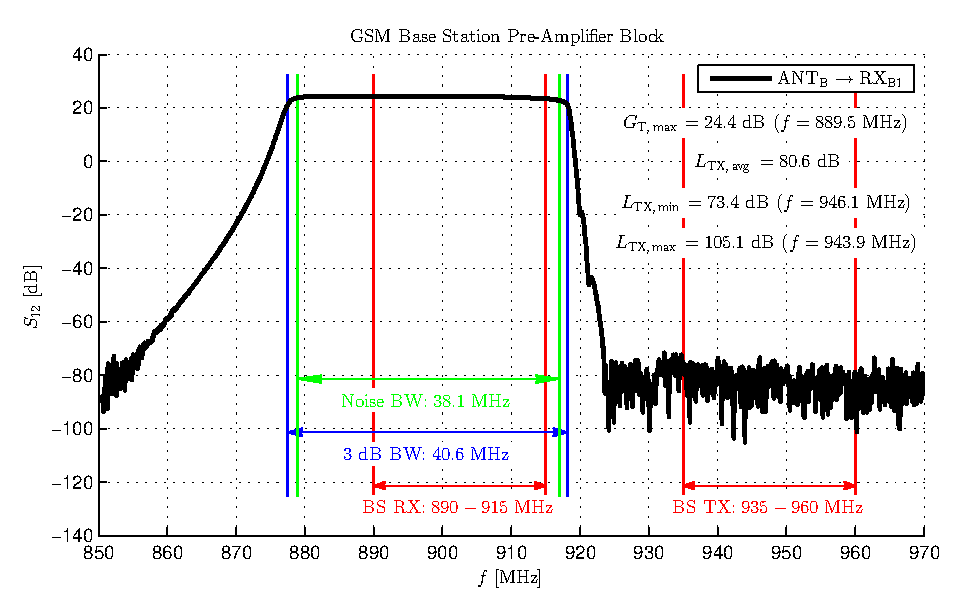
\epsfig{file=img/s12.eps, width=\textwidth}
	\caption{Results from the diplexer characterization.}
	\label{f:r1}
	\end{center}
	\vspace*{-12pt}
\end{figure}


\subsection{Noise temperature of the RX pre-amplifier block}

\textit{Determine the noise temperature of the RX block (consisting of bias tee, 
diplexer and pre-amplifier) with the Y-coefficient method. Use the noise diode 
as active noise source (and as passive noise source at room temperature when 
supply voltage is switched off).}

\vspace*{\oneLine}
\noindent
Text here.

\begin{figure}[h!]
	\begin{center}
	\setlength{\unitlength}{1mm}
	\begin{picture}(168, 13)
		\linethickness{0.2mm}
		\put(0, 0.4){\framebox[10mm]{$V_\mathrm{DC}$}}
		\put(10, 1.4){\vector(1,0){20}}
		\put(30, 0){\framebox[25mm]{Noise diode}}
		\put(55, 1.4){\vector(1,0){25}}
		\put(80, 0.4){\framebox[28mm]{$\mathrm{ANT} \rightarrow \mathrm{RX}_1$}}
		\put(108, 1.4){\vector(1,0){20}}
		\put(128, 0.4){\framebox[40mm]{Sprectrum analyzer}}
		
		%\put(20, 4){\makebox(0,0){Cable}}
		\put(67.5, 8){\makebox(0,0){Direct}}
		\put(67.5, 4){\makebox(0,0){connection}}
		%\put(118, 4){\makebox(0,0){Cable}}
		\put(94, 7){\makebox(0,0){DDU module}}
	\end{picture}
	\vspace*{\halfLine}
	\caption{Noise temperature measurement setup}
	\label{f:m3}
	\end{center}
	\vspace*{-12pt}
\end{figure}


\subsection{Sensitivity of the RX pre-amplifier block}

\textit{Measure the sensitivity of the RX block using suitable equipment.}

\vspace*{\oneLine}
\noindent
Text here.

\begin{figure}[h!]
	\begin{center}
	\setlength{\unitlength}{1mm}
	\begin{picture}(167, 13)
		\linethickness{0.2mm}
		\put(0, 0.4){\framebox[34mm]{Signal generator}}
		\put(34, 1.4){\vector(1,0){14}}
		\put(48, 0){\framebox[23mm]{Attenuator}}
		\put(71, 1.4){\vector(1,0){14}}
		\put(85, 0.4){\framebox[28mm]{$\mathrm{ANT} \rightarrow \mathrm{RX}_1$}}
		\put(113, 1.4){\vector(1,0){14}}
		\put(127, 0.4){\framebox[40mm]{Sprectrum analyzer}}
		
		%\put(41, 4){\makebox(0,0){Cable}}
		%\put(78, 4){\makebox(0,0){Cable}}
		%\put(120, 4){\makebox(0,0){Cable}}
		\put(99, 7){\makebox(0,0){DDU module}}
		\put(66.5, 8){\makebox(0,0){$\overbrace{\hspace*{35mm}}^\textrm{only if needed}$}}
	\end{picture}
	\vspace*{\halfLine}
	\caption{Measurement setup used in the sensitivity measurement.}
	\label{f:m4}
	\end{center}
	\vspace*{-12pt}
\end{figure}


\newpage
\section{Pre-study calculations and related tasks}

The following subsections will present answers to pre-study tasks $2.2 - 2.4$.


\subsection{Mismatch attenuation}

\textit{A signal generator is connected to the input of the RX pre-amp block. 
The VSWR (voltage standing wave ratio) of the pre-amp is 2.0 and the VSWR of 
the output of the signal generator is 1.6.
\vspace*{-\halfLine}
\begin{enumerate}[label=\alph*), itemsep=0pt]
\item What is the range of additional attenuation due to this mismatch in 
	the measurement of the pre-amp block?
\item In what range is the attenuation due to mismatch, when an ideal 10 dB 
	attenuator is connected between the signal generator and the pre-amp block? 
	What is the benefit/drawback of inserting this attenuator?
\end{enumerate}}
		
\vspace*{\halfLine}
\noindent
Text here.


\subsection{Noise temperature}

\textit{The noise temperature of the pre-amp block is determined using the 
Y-coefficient method. The noise level of the spectrum analyzer HP8596E is 
$P_\mathrm{SA} < -125$~dBm when the input is matched and the resolution 
bandwidth is 30~Hz.
\vspace*{-\halfLine}
\begin{enumerate}[label=\alph*), itemsep=0pt]
\item How much gain is required from the LNA in order to measure the noise 
	temperature with the HP8596E? The noise figure of the amplifier is 2.8~dB 
	and the attenuation of the bias Tee and the diplexer is 0.7~dB and 0.4~dB, 
	respectively.
\item Does the order (i.e. which is first in the chain) of the amplifier, 
	bias tee and the diplexer in the pre-amp block have any influence on the 
	result of Y-coefficient measurement? If yes, say why.
\end{enumerate}}

\vspace*{\halfLine}
\noindent
Text here.


\subsection{Requirements with evolving standards}

\textit{Discuss briefly the major changes in the requirements for the 
RF performance of the blocks in the RX chain when we move from 2G to 
3G to 4G systems.}

\vspace*{\oneLine}
\noindent
Text here.


\begin{thebibliography}{9}%\itemsep 7pt\parskip -5pt 

\bibitem{hs} $\mathrm{Huber}+\mathrm{Suhner}$, 
	\textit{RF Cables}, 
	Edition 2013/09. 
	Available online at \href{http://ipaper.ipapercms.dk/HUBERSUHNER/Technologies/Radiofrequency/RFCablesEN/}
		{\texttt{http://ipaper.\linebreak{}ipapercms.dk/HUBERSUHNER/Technologies/Radiofrequency/RFCablesEN/}}
	[Retrieved: January 10th, 2014].


\bibitem{pozar} D.\ M.\ Pozar, 
	\textit{Microwave Engineering}, 
	J.\ Wiley \& Sons, 4th Ed., 2012. 
	ISBN: 978-0-470-63155-3.
	
%\bibitem{gains} J.\ C.\ Logan, J.\ W.\ Rockway, 
%	``Dipole and Monopole Antenna Gain and Effective Area for Communication Formulas.''
%	Available online at \url{www.dtic.mil/cgi-bin/GetTRDoc?AD=ADA332891}
%	[Retrieved: November 25th, 2013].

\bibitem{parts} M.\ Steer, 
	\textit{Microwave and RF Design -- A Systems Approach}, 
	SciTech Publishing, 2010. 
	ISBN: 978-1-891-12188-3.
	
%\bibitem{kandi} T.\ Leinonen, 
% 	``Antenna and front-end challenges for mobile software-defined radio receiver,''
%	B.\ Sc.\ (Tech.) thesis (in Finnish), 2012. 
% 	Available online at \url{http://urn.fi/URN:NBN:fi:aalto-201301161154}.
	
%\bibitem{iet} R.\ J.\ Collier, A.\ D.\ Skinner (editors), 
%	\textit{Microwave Measurements}, 
%	The Institution of Engineering and Technology, 3rd Ed., 2007. 
% 	ISBN: 978-0-86341-735-1.

\end{thebibliography}

\end{document}
